\chapter{Resultados}
\label{ch:resultados}

Neste cap�tulo ser�o apresentados exemplos e resultados obtidos utilizando a metodologia e o programa computacional descritos nos cap�tulos anteriores.

\section{Problemas El�pticos}
\label{sc:elipticos}
Este se��o tem por objetivo principal avaliar a resolu��o da equa��o de press�o, a qual para o caso de estado estacion�rio, pode ser considerada uma t�pica equa��o el�ptica.

\subsection{Permeabilidade Homog�nea}
\label{sc:homogenea}
Para casos no qual o campo de permeabilidade n�o varia ao longo do dom�nio, podemos dizer que o mesmo � homog�neo.

\begin{figure}
\centering
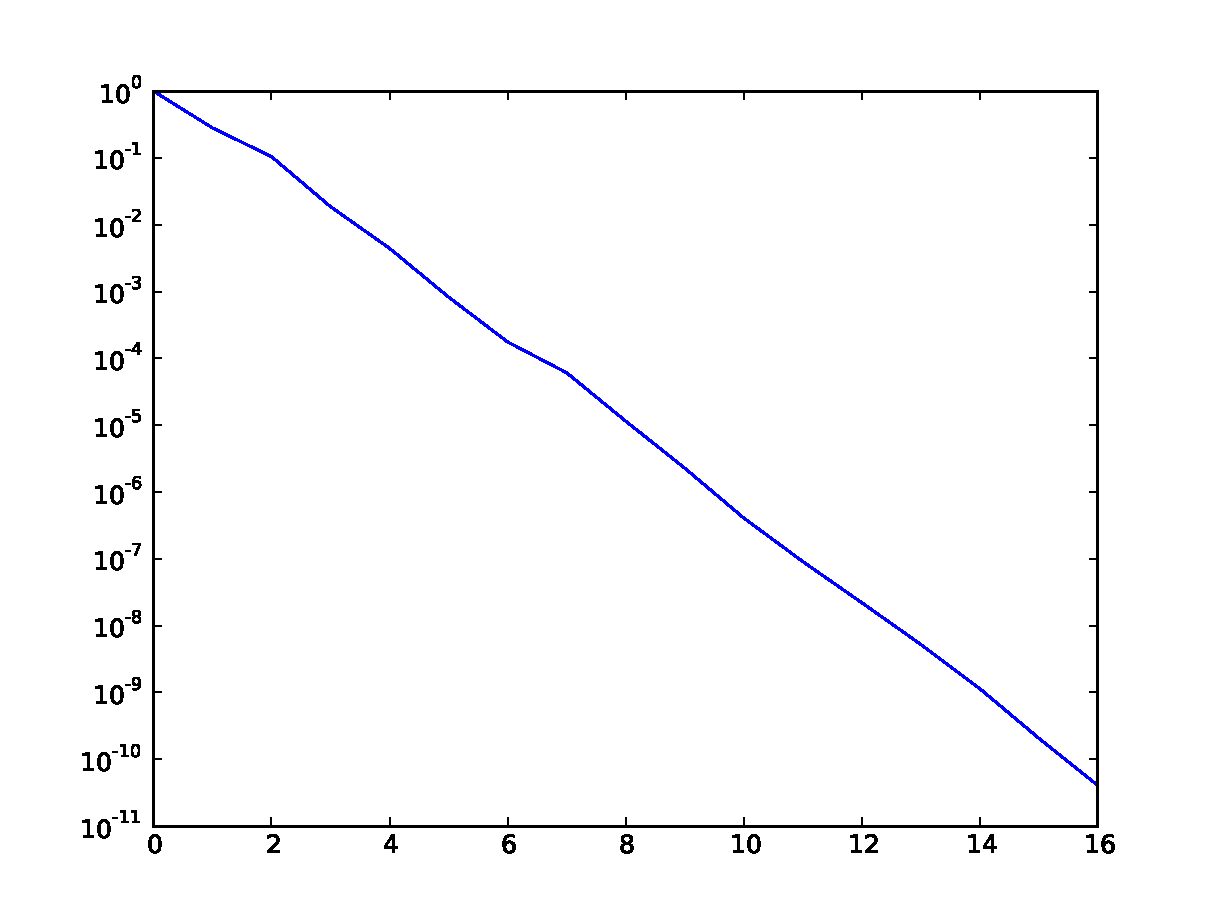
\includegraphics[width=0.5\textwidth]{chapters/ch05/residuals_ex02.pdf}
\caption[Res�duo para problema homog�nio com tensor cheio]{Res�duo obtido para o problema homog�neo com o tensor cheio.}
\label{fig:residuals_ex02}
\end{figure}

Para o exemplo 02 retirado de \citep{Silva2008}, a evolu��o do res�duo pode ser vista na figura~\ref{fig:residuals_ex02}

\subsection{Permeabilidade Heterog�nea}
\label{sc:heterogenea}
Em um caso real, as propriedades da rocha ir�o variar ao longo do dom�nio, resultando em um caso heterog�neo.


